\section{Robot Design}
\subsection{Component Identification and Selection}
A critical aspect of the progress has been the careful selection of internal components that will drive the core functionality of the robot. After thorough research and evaluation, the following essential components have been identified:
\begin{itemize}
    \item \textbf{NVIDIA Jetson Orin Nano (x1):} Serves as the primary processing unit
    \item \textbf{Speaker (x1):} Enables the robot to deliver audio feedback and engage in voice-based communication with users.
    \item \textbf{Pressure Sensors (x2):} Integrated for tactile responsiveness, allowing the robot to detect touch and adjust interactions based on user input.
    \item \textbf{Microphones (x2):} Facilitate audio input for natural language processing and communication.
    \item \textbf{Servo Motors (x5):} Power the robot's neck and arm movement.
    \item \textbf{Camera (x1):} Provides visual input.
\end{itemize}

\subsection{Design Development}
The cornerstone of progress has been the development of the robot's overall design. The concept revolves around an anthropomorphic robot inspired by a red panda, aimed at creating a visually appealing and emotionally engaging design.

\begin{figure}[ht]
    \centering
    \captionsetup{justification=centering}
    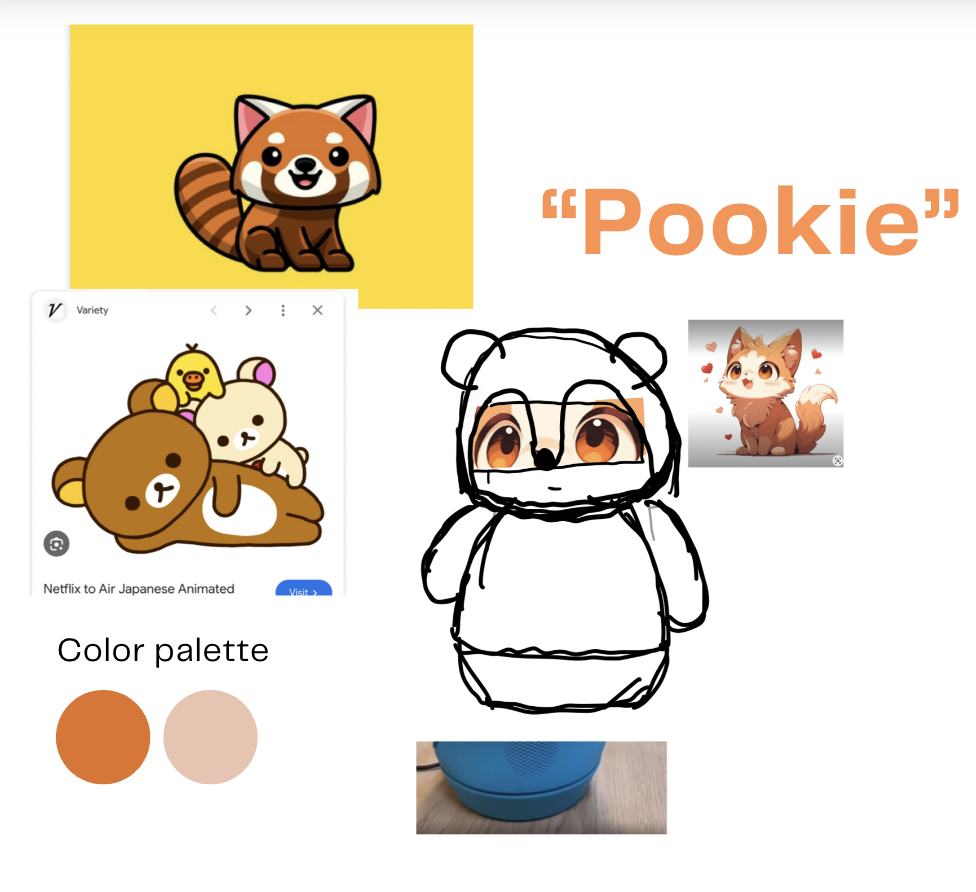
\includegraphics[width=0.75\textwidth]{design.png}
    \caption{Pookie Anthropomorphic Design}
    \label{fig:design}
\end{figure}

Fusion 360 was utilized to visualize and refine the concept, creating a preliminary sketch of the robot. This 3D modeling software facilitated the determination of precise dimensions and allowed for quick iterations on different design elements. Various body proportions were explored, with features adjusted to achieve a balance between animal-like charm and human-like functionality.

The design process involved crafting an external shell while simultaneously considering the internal layout. This approach ensured that all previously selected components could be accommodated within the shell while maintaining the desired aesthetics.

\begin{figure}[ht]
    \centering
    \captionsetup{justification=centering}
    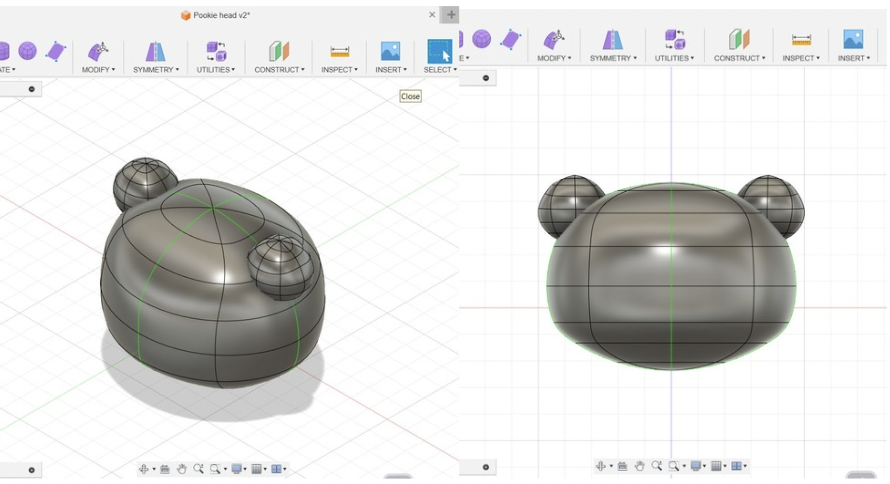
\includegraphics[width=0.85\textwidth]{head.png}
    \caption{Pookie’s Head Shell Design in Fusion360}
    \label{fig:head}
\end{figure}

\begin{figure}[ht]
    \centering
    \captionsetup{justification=centering}
    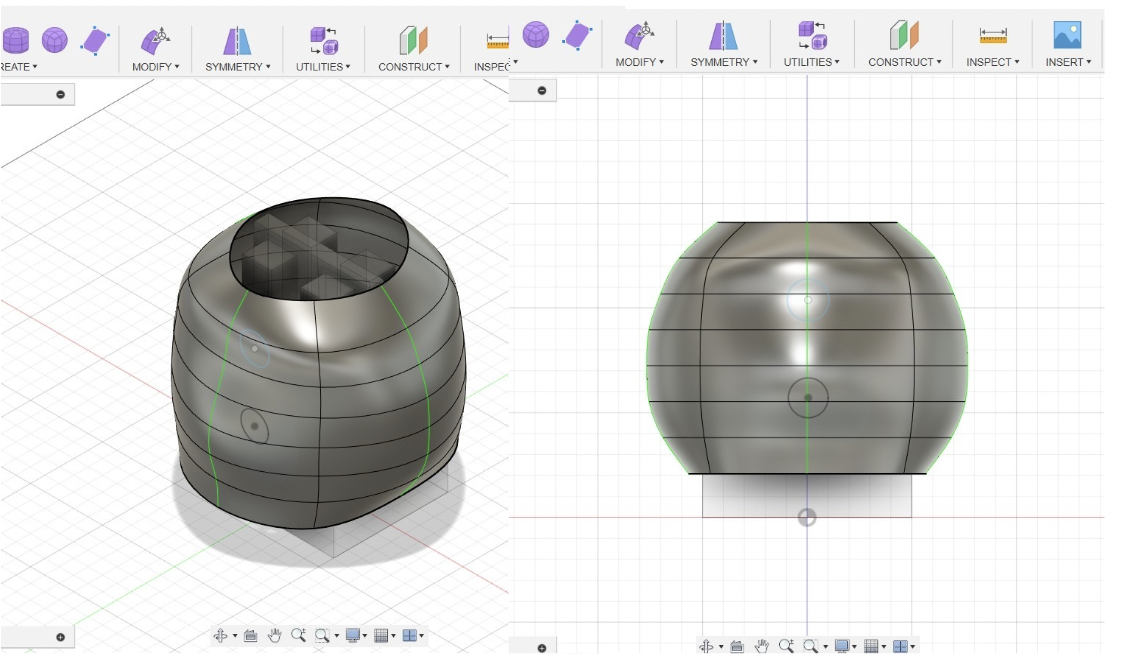
\includegraphics[width=0.85\textwidth]{body.png}
    \caption{Pookie’s Body Shell Design in Fusion360}
    \label{fig:body}
\end{figure}

Careful consideration was given to the robot's dimensions, aiming for a scale that would make it approachable yet large enough to house all necessary components and facilitate meaningful interactions. This iterative process resulted in a comprehensive 3D model that serves as an initial blueprint for Pookie the robot. 

\begin{figure}[ht]
    \centering
    \captionsetup{justification=centering}
    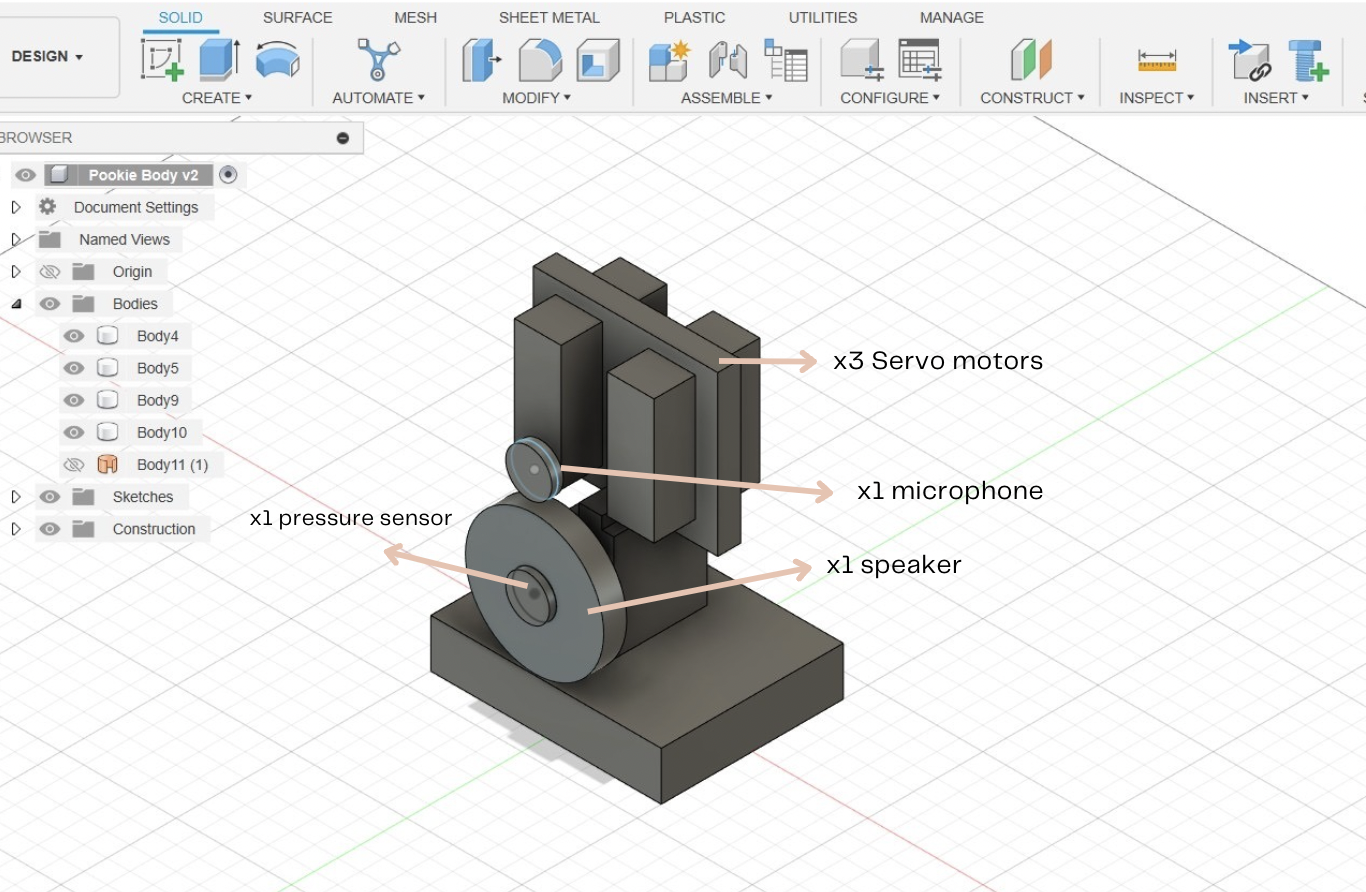
\includegraphics[width=0.85\textwidth]{inside.png}
    \caption{Component Dimensions Inside Pookie’s Body Shell}
    \label{fig:inside}
\end{figure}

\newpage
\subsection{Eyes Design}
The robot's eye design is crucial for conveying emotion and engaging users. After reviewing numerous examples, optimal designs were selected based on their potential to humanize the robot and facilitate non-verbal communication. The selected LED eye designs are expected to integrate seamlessly with other expressive features, contributing significantly to creating a cohesive and engaging interaction experience.
\begin{figure}[ht]
    \centering
    \captionsetup{justification=centering}
    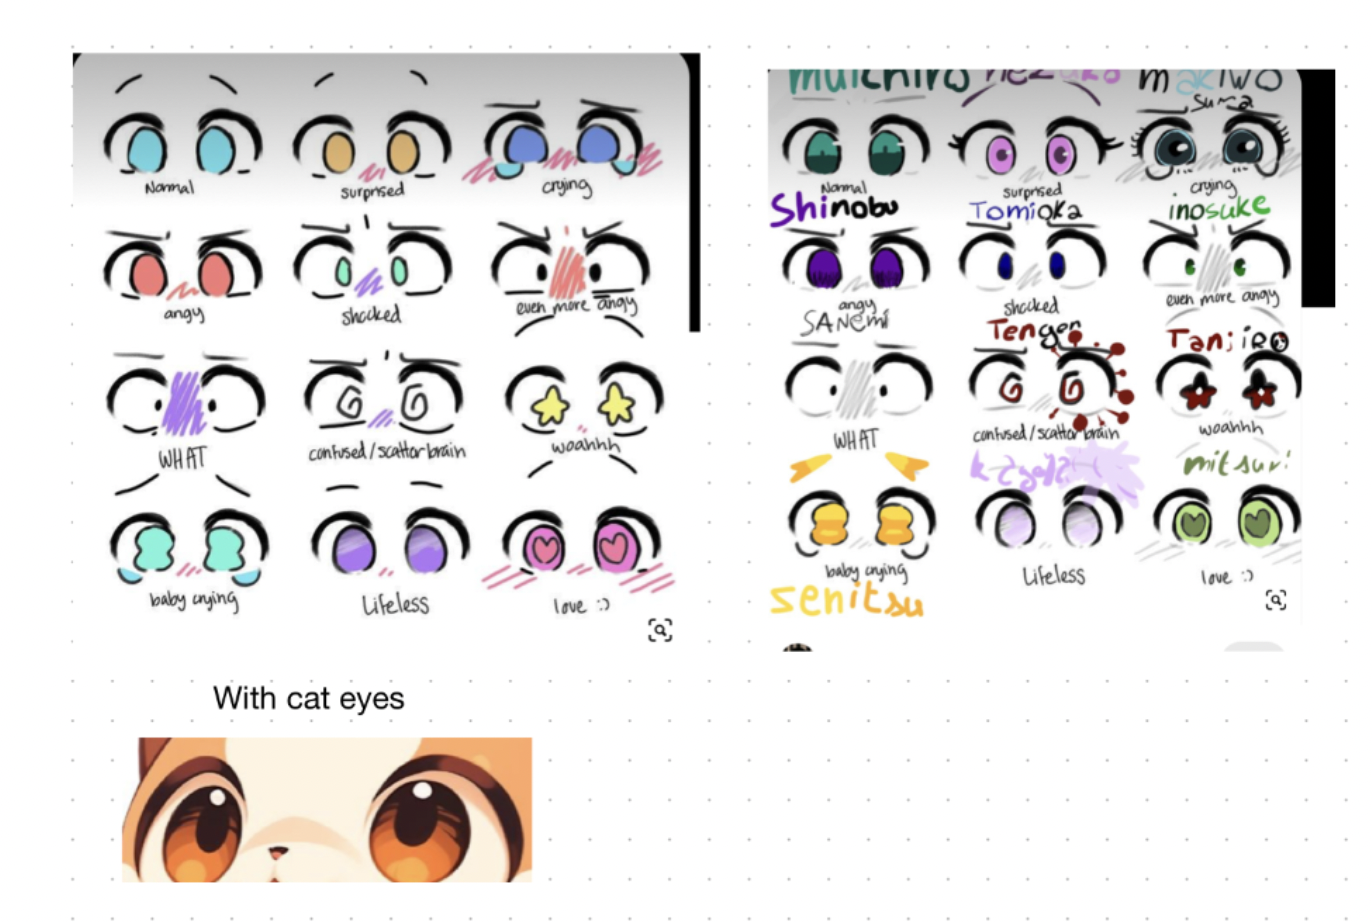
\includegraphics[width=0.75\textwidth]{eyes.png}
    \caption{Pookie's LED Eye Design}
    \label{fig:eyes}
\end{figure}

\subsection{Emotion Expression through Movement}
The project has progressed to developing expressive movement patterns, enabling the robot to convey a spectrum of emotions through physical gestures. This phase involves mapping specific combinations of head tilts, body postures, and limb movements to effectively communicate various emotional states such as happiness, curiosity, confusion, and alertness. 
